%-------------------------------------------------------------------------------

% CHAPTER 12

%-------------------------------------------------------------------------------

\chapter[Method of characteristics, I]{Method of characteristics, I: Linear case}

Over the next two chapters we will develop a method for solving first order PDEs called the method of characteristics. In this chapter we will restrict attention to inhomogeneous linear equations (first with constant coefficients, then with nonconstant coefficients) where the method of characteristics boils down to finding a sensible change of coordinates after which the PDE looks much simpler.

\section{Linear change of coordinates}\label{sct:linearcoord}

Occasionally, for very simple PDEs, one can change coordinates and turn them into PDEs we already know how to solve.

\subsection{Examples}
\begin{exm}
Consider the PDE for $\phi(x,y)$:
\[\frac{\partial\phi}{\partial x}=0.\]
This says $\phi$ is constant in the $x$-direction, so $\phi$ is a function of $y$ alone. Any function of $y$ is a solution, i.e. $\phi(x,y)=C(y)$ where $C$ is an arbitrary function.
\end{exm}
\begin{exm}
Consider the PDE for $\phi(x,y)$:
\[\frac{\partial\phi}{\partial x}-\frac{\partial\phi}{\partial y}=0.\]
The expression on the left-hand side looks like the expression
\[\pd{\phi}{u}=\pd{x}{u}\pd{\phi}{x}+\pd{y}{u}\pd{\phi}{y}\]
coming from the chain rule, provided we pick
\[\pd{x}{u}=1,\qquad\pd{y}{u}=-1.\]
So let's change to a new (linear) system of coordinates $(u,v)$ satisfying
\[\pd{x}{u}=1,\qquad\pd{y}{u}=-1.\]
For example we could take
\[\twob{x}{y}=\matr{1}{0}{-1}{1}\twob{u}{v}\]
or
\[\twob{x}{y}=\matr{1}{7}{-1}{0}\twob{u}{v}.\]
The only conditions for this to define a suitable coordinate change are:
\begin{itemize}
\item that the first column is given by $1$ and $-1$ (the coefficients of $\pd{\phi}{x}$ and $\pd{\phi}{y}$ in the equation),
\item that the matrix is invertible.
\end{itemize}
Let's use
\[\twob{x}{y}=\matr{1}{0}{-1}{1}\twob{u}{v}\]
whose inverse is
\[\twob{u}{v}=\matr{1}{0}{1}{1}\twob{x}{y}\]
With respect to the new basis, the chain rule tells us that
\begin{align*}
\pd{\phi}{u}&=\pd{x}{u}\pd{\phi}{x}+\pd{y}{u}\pd{\phi}{y}\\
            &=\pd{\phi}{x}-\pd{\phi}{y}\\
            &=0\mbox{ (by our equation)}
\end{align*}
so the general solution to the equation is $\phi(u,v)=C(v)$. In terms of the original basis this is $\phi(x,y)=C(x+y)$. So any function of $v=x+y$ is a solution. For example $\sin(x+y)$, $e^{7(x+y)}$,...
\end{exm}
\begin{exm}
Consider the PDE for $\phi(x,y)$:
\[\frac{\partial\phi}{\partial x}-\frac{\partial\phi}{\partial y}=x.\]
If we make the same change of coordinates as before,
\[\twob{x}{y}=\matr{1}{0}{-1}{1}\twob{u}{v},\qquad \twob{u}{v}=\matr{1}{0}{1}{1}\twob{x}{y}\]
this equation becomes
\begin{align*}
\pd{\phi}{u}&=\pd{x}{u}\pd{\phi}{x}+\pd{y}{u}\pd{\phi}{y}\\
            &=\pd{\phi}{x}-\pd{\phi}{y}\\
            &=x\mbox{ (by our equation)}\\
            &=u\mbox{ (by our coordinate change).}
\end{align*}
We can integrate this and get
\[\phi(x,y)=\frac{1}{2}u^2+C(v)\]
where $C(v)$ is an arbitrary function of $v=x+y$. Translating back into our original coordinates we get
\[\phi(x,y)=\frac{x^2}{2}+C\left(x+y\right).\]
\end{exm}
\subsection{In general}
This trick works with any PDE for $\phi(x_1,\ldots,x_n)$ of the form
\[\sum_{i=1}^nA_i\frac{\partial\phi}{\partial x_i}=0\]
In new coordinates $(u_1,\ldots,u_n)$, we have
\[\pd{\phi}{u_1}=\sum_{i=1}^n\pd{x_i}{u_1}\pd{\phi}{x_i}\]
so $\pd{\phi}{u}=\sum A_i\pd{\phi}{x_i}$ if $\pd{x_i}{u_1}=A_i$. A suitable linear change of coordinates is therefore
\[\left(\begin{array}{c}
x_1\\
\vdots\\
x_n
\end{array}\right)=\left(\begin{array}{ccc}A_1 & \star & \star\\
\vdots & \vdots & \vdots\\
A_n & \star & \star\end{array}\right)\left(\begin{array}{c}u_1\\ \vdots\\ u_n\end{array}\right)\]
where the stars can be anything, provided the matrix is invertible. With this change of coordinates, the chain rule tells us that
\[\pd{\phi}{u}=\sum A_i\pd{\phi}{x_i}\]
so the solution to the equation $\sum A_i\pd{\phi}{x_i}=0$ is
\[C(u_2,\ldots,u_n)\]
for an arbitrary function $C$.

\begin{exm}
Consider the equation
\[\pd{\phi}{x}+2\pd{\phi}{y}=\sin y.\]
Use the coordinate change
\[\twob{x}{y}=\matr{1}{0}{2}{1}\twob{u}{v}\]
whose inverse is
\[\twob{u}{v}=\matr{1}{0}{-2}{1}\twob{x}{y}.\]
The chain rule tells us that
\begin{align*}
\pd{\phi}{u}&=\pd{x}{u}\pd{\phi}{x}+\pd{y}{u}\pd{\phi}{y}\\
            &=\pd{\phi}{x}+2\pd{\phi}{y}\\
            &=\sin y\\
            &=\sin(2u+v).
\end{align*}
Then, fixing $v$ and integrating with respect to $u$, we get
\[\phi(u,v)=-\frac{1}{2}\cos(2u+v)+C(v)\]
or
\[\phi(x,y)=-\frac{1}{2}\cos y+C(y-2x).\]
\end{exm}

\subsection{Boundary conditions}

If we want to fix the arbitrary function $C$ then we need more information.

\begin{exm}
{\bf Solve the equation
\[\pd{\phi}{x}+2\pd{\phi}{y}=\sin y\]
subject to the boundary condition $\phi(s,0)=s^2$.}

We have already seen that the general solution to this equation is $\phi(x,y)=-\frac{1}{2}\cos y+C(y-2x)$. If we substitute this into the boundary condition then we get
\[s^2=-\frac{1}{2}\cos(0)+C(0-2s)\]
which means
\[C(-2s)=s^2+\frac{1}{2}.\]
Substituting $w=-2s$ ($s=-w/2$) gives
\[C(w)=\frac{w^2}{4}+\frac{1}{2}.\]
\end{exm}

\section{Nonlinear change of coordinates}

We have only allowed ourselves to change coordinates by a linear transformation. What kind of equations do we get if we make more interesting coordinate changes?

\subsection{An elementary example}

\begin{exm}
Use plane polar coordinates:
\begin{align*}
x&=r\cos\theta\\
y&=r\sin\theta.
\end{align*}
By the chain rule we have
\begin{align*}
\frac{\partial\phi}{\partial r}&=\frac{\partial\phi}{\partial x}\frac{\partial x}{\partial r}+\frac{\partial\phi}{\partial y}\frac{\partial y}{\partial r}\\
&=\frac{x}{r}\frac{\partial\phi}{\partial x}+\frac{y}{r}\frac{\partial y}{\partial r}
\end{align*}
In particular, the equation
\[\frac{\partial\phi}{\partial r}=0\]
becomes (after multiplying out by $r$)
\begin{equation}\label{eqn-radial-pde-exm}x\frac{\partial\phi}{\partial x}+y\frac{\partial\phi}{\partial y}=0.\end{equation}
In particular, the solutions to Equation \eqref{eqn-radial-pde-exm} are just functions of $\theta=\tan^{-1}(y/x)$. For instance, $\tan(\theta)=y/x$ is a solution (away from $x=0$) or $\cos\theta=x/\sqrt{x^2+y^2}$ is a solution. (Check them!)
\end{exm}

\subsection{Characteristic vector field}

\begin{lma}\label{lma:chain}
Given an expression of the form
\[\sum_{i=1}^nA_i(x_1,\ldots,x_n)\frac{\partial\phi}{\partial x_i},\]
suppose that we can find coordinates $(u_1,\ldots,u_n)$ such that
\[\pd{x_i}{u_1}=A_i(x_1,\ldots,x_n).\]
Then
\[\pd{\phi}{u}=\sum_{i=1}^nA_i(\vec{x})\pd{\phi}{x_i}.\]
\end{lma}
\begin{proof}
This is immediate from the chain rule:
\[\pd{\phi}{u}=\sum_{i=1}^n\pd{x_i}{u_1}\pd{\phi}{x_i}=\sum_{i=1}^nA_i(\vec{x})\pd{\phi}{x_i}.\]
\end{proof}

In fact we can always find suitable coordinates, at least locally. So how do we solve the equations
\[\pd{x_i}{u_1}=A_i(x_1,\ldots,x_n)?\]

\begin{exm}
Consider the equation $x\pd{\phi}{x}+y\pd{\phi}{y}=0$. We want to solve
\[\twob{\pd{x}{u}}{\pd{y}{u}}=\twob{x}{y}.\]
For simplicity, let's write this as
\[\twob{\dot{x}}{\dot{y}}=\twob{x}{y}.\]
The solution is $x=Ae^u$, $y=Be^u$. We want to think of these two equations as giving a coordinate transformation, but we have three new coordinates $u,A,B$, so this doesn't quite make sense yet. Let us make an arbitrary choice: set $A=1$ and take our new coordinates to be $u$ and $v=A$. That is:
\[x=e^u,\qquad y=ve^u.\]
The inverse of this coordinate transformation is
\[u=\ln x,\qquad v=y/x.\]
This arbitrary choice is completely analogous to the way we could choose our matrix entries freely in Section \ref{sct:linearcoord}. With these new coordinates, we have
\[x\pd{\phi}{x}+y\pd{\phi}{y}=\pd{\phi}{u}\]
by Lemma \ref{lma:chain}. Therefore the equation is $\pd{\phi}{u}=0$ and the solution is $\phi(u,v)=C(v)$ (where $C$ is an arbitrary function). Substituting our expression $v=y/x$ we get
\[\phi(x,y)=C(y/x).\]
\end{exm}

\begin{dfn}
Consider an equation of the form $A(x,y)\pd{\phi}{x}+B(x,y)\pd{\phi}{y}+C(x,y)\phi+D(x,y)=0$ (``inhomogeneous linear''). The vector field
\[\twob{A(x,y)}{B(x,y)}\]
is called the characteristic vector field. The differential equations
\[\twob{\dot{x}}{\dot{y}}=\twob{A(x,y)}{B(x,y)}\]
are called the characteristic equations and a curve $(x(u),y(u))$ satisfying the characteristic equations is called a characteristic curve (it is always tangent to the characteristic vector field). This method for solving first order PDEs is called the {\em method of characteristics}.
\end{dfn}

\begin{rmk}
In general, if you have a vector field $(A(x,y),B(x,y))$ and a curve satisfying
\[\dot{x}=A(x,y),\qquad \dot{y}=B(x,y)\]
then the curve is called an {\em integral curve} (it's found by integrating (i.e. solving) these differential equations). I may occasionally slip and use this terminology, so it's best that you're aware of it.
\end{rmk}

\begin{exm}
Consider the equation
\[-y\pd{\phi}{x}+x\pd{\phi}{y}=0.\]
The characteristic vector field is $(-y,x)$ and the characteristic equations are
\[\dot{x}=-y,\qquad\dot{y}=x.\]
Differentiating again we get $\ddot{x}=-x$, so $x=A\cos u+B\sin u$ and $y=-\dot{x}=A\sin u-B\cos u$. Let us pick $B=0$ and $v=A$. Now we have
\[(x,y)=(v\cos u,v\sin u).\]
The inverse coordinate transform is
\[v=\sqrt{x^2+y^2},\qquad u=\tan^{-1}(y/x).\]
The equation becomes $\pd{\phi}{u}=0$ which has solution $C(v)=C(\sqrt{x^2+y^2})$.
\end{exm}

{
\begin{center}
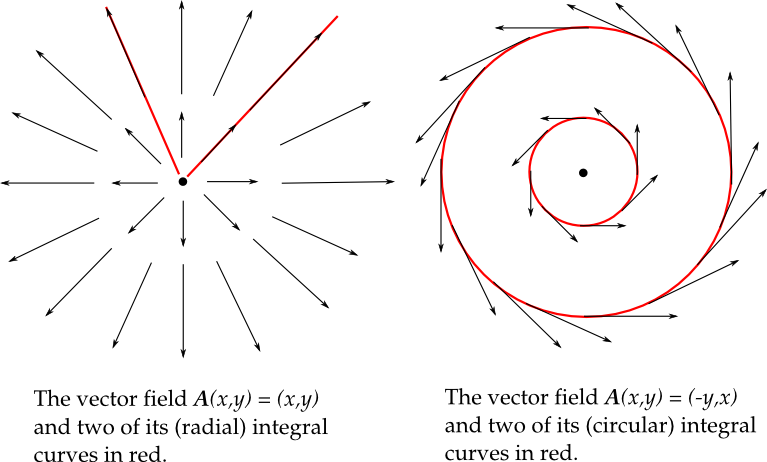
\includegraphics[width=400px]{integral-curves.png}
\end{center}
}

\begin{exm}
Consider the equation
\begin{equation}\label{eqn-pde-characteristic-exm}x\frac{\partial\phi}{\partial x}-\frac{\partial\phi}{\partial y}=0.\end{equation}
The characteristic vector field in this equation is $(x,-1)$. The characteristic curves $(x(u),y(u))$ are solutions to
\[\dot{x}=x,\ \dot{y}=-1.\]

{
\begin{center}
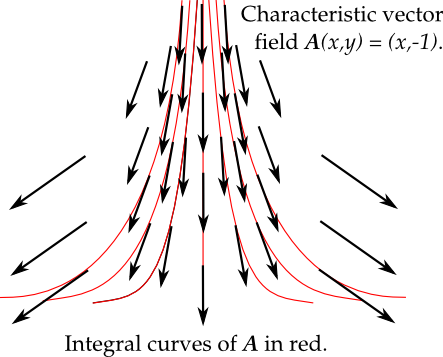
\includegraphics[width=250px]{characteristics2.png}
\end{center}
}

These equations have solution
\[x=Ae^u,\qquad y=B-u\]
Pick $B=0$ and $v=A$. The new coordinates are therefore
\begin{align*}
x&=ve^u,&y&=-u\\
u&=-y,&v&=xe^y.
\end{align*}

{
\begin{center}
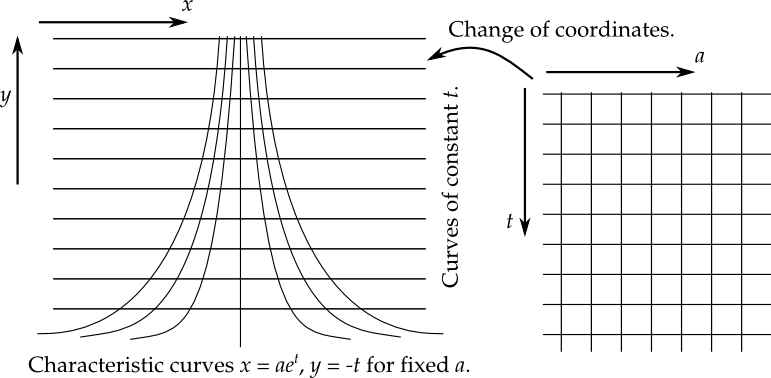
\includegraphics[width=400px]{characteristics1.png}
\end{center}
}

Lemma \ref{lma:chain} tells us that
\[\pd{\phi}{u}=x\pd{\phi}{x}-\pd{\phi}{y}\]
so Equation \eqref{eqn-pde-characteristic-exm} becomes $\pd{\phi}{u}=0$ and has solution $\phi(u,v)=C(v)$. In other words, $\phi(x,y)=C(xe^y)$.
\end{exm}

\begin{rmk}\label{rmk:bequalszero}
How did we make this choice $B=0$? Since $y=B-u$ we could always achieve $B=0$ by translating in the $t$ coordinate, that is using the new $u$-coordinate $\tilde{u}=u-B$, in terms of which $y=-\tilde{u}$. If we had picked $A=0$, $B=v$ then the corresponding ``change of coordinates'' would have been $x=0$, $y=v-u$, which isn't really a change of coordinates because you can never express points with $x\neq 0$ in terms of $u$ and $v$.
\end{rmk}

\begin{exm}
To illustrate what happens for different choices, let's work through what would have happened if we had picked $A=1$, $B=v$ in the previous example. The corresponding change of coordinates would have been $x=e^u$, $y=v-u$. The equation has solution $\tilde{C}(v)=\tilde{C}(y+\ln x)$. This looks different from the previous answer, but notice that $y+\ln x=\ln(xe^y)$, so they're really the same solution in disguise! In particular, if you take $\tilde{C}(v)=C(e^v)$ then you really have the same solution. Going backwards, $C(v)=\tilde{C}(\ln v)$ gives a correspondence between solutions, but notice that this only makes sense when $v>0$. Indeed, if you look at the coordinates defined by $x=e^u$, $y=v-u$, you can see that these coordinates only cover the region $x>0$.
\end{exm}

\begin{rmk}
In summary, this solution is just as valid as the previous solution, but you should be careful to point out that the solution is only defined on the region $x>0$ of the plane. In general, choosing which constants of integration to use as coordinates requires some thought specific to the problem at hand. You may need to use different choices to cover different regions of the plane. You will build up a feeling for which choices are sensible by working with examples. Sometimes you can say ``without loss of generality we can set $B=0$'' (or something like that) as in Remark \ref{rmk:bequalszero} but often you just have to make a judicious choice.
\end{rmk}

\section{More examples}

\begin{exm}
Consider the PDE for $\phi(x,y)$:
\[\frac{1}{x}\frac{\partial\phi}{\partial x}-y\frac{\partial\phi}{\partial y}=0.\]
The characteristic vector field is $(1/x,-y)$ so the characteristic curves satisfy
\[\dot{x}=1/x,\ \dot{y}=-y.\]
The first equation can be rearranged as $x\dot{x}=1$ or $\frac{1}{2}\pd{x^2}{u}=1$ so $x=\sqrt{2u+A}$. The second equation has solution $y=Be^{-u}$. We can reparametrise $u$ to $\tilde{u}=u-A/2$ so that without loss of generality $A=0$. Our new coordinates are therefore $(u,v)$ where $u=x^2/2$ and $v=B=ye^u=ye^{x^2/2}$. In these new coordinates the PDE becomes
\[\frac{\partial\phi}{\partial u}=0\]
so solutions to the PDE are just arbitrary functions of $v=ye^{x^2/2}$.
\end{exm}
\begin{exm}
Consider the PDE for $\phi(x,y)$:
\[\frac{1}{x}\frac{\partial\phi}{\partial x}-y\frac{\partial\phi}{\partial y}=y.\]
The characteristic vector field and characteristic curves are the same as in the previous example so our new coordinates are again $(u,v)=(x^2/2,ye^{x^2/2})$. In these new coordinates the equation becomes
\[\frac{\partial\phi}{\partial t}=y=ve^{-u}.\]
Integrating this we get
\[\phi(u,v)=-ve^{-u}+C(v)\]
for some arbitrary function $C$. In other words, returning to our original coordinates,
\[\phi(x,y)=-y+C(ye^{x^2/2}).\]
\end{exm}
\begin{exm}
Consider the PDE for $\phi(x,y)$:
\[\frac{\partial\phi}{\partial x}+2x\frac{\partial\phi}{\partial y}=1.\]
The characteristic vector field is $(1,2x)$ so the characteristic curves satisfy
\[\dot{x}=1,\ \dot{y}=2x,\]
thus $x=u+A$ and $y=(u+A)^2+B$. Reparametrising so that $A=0$ and setting $v=B$, we get $(x,y)=(u,u^2vB)$ or $(u,v)=(x,y-x^2)$ as our change of coordinates. The PDE becomes
\[\frac{\partial\phi}{\partial u}=1\]
so $\phi(u,v)=u+C(v)$ for some arbitrary function $C$. In other words,
\[\phi(x,y)=x+C(y-x^2).\]
\end{exm}
\begin{exm}
Consider the PDE for $\phi(x,y)$:
\[y\frac{\partial\phi}{\partial x}+x\frac{\partial\phi}{\partial y}=0.\]
The characteristic vector field is $(y,x)$ so the characteristic curves satisfy
\[\dot{x}=y,\ \dot{y}=x\]
Differentiating with respect to $u$ again we get $\ddot{x}=x$ so $x=Ae^u+Be^{-u}$. Since $y=\dot{x}$ we have $y=Ae^u-Be^{-u}$. If we want to understand these curves geometrically, notice that $x^2-y^2=4AB$ so if $AB$ is fixed then the characteristic curves are hyperbolae.

There is no single choice like $A=0$ or $B=0$ which will give us a good coordinate system everywhere. If there were we would be able to change coordinates and make the hyperbolae look like a family of parallel lines, but the hyperbola $x^2-y^2=0$ consists of two straight lines intersecting at a point, which can never be made to look like a single straight line!

If we pick $A=0$ or $B=0$ then we can only ever hope for our coordinates to to cover points on the hyperbola $x^2-y^2=4ab=0$, so we should pick a nonzero value for $A$ or $B$.

We will try fixing $B=1$, $A=v$, so $x=ve^u+e^{-u}$ and $y=ve^u-e^{-u}$. As expected, this choice of coordinates does not cover the whole plane: $x-y=2e^{-u}$ is always positive so we can only cover the part of the plane to the right of the line $y=x$. But at least that is a large open subset. With this choice, $u=-\ln\left(\tfrac{1}{2}(x-y)\right)$ and $v=(x^2-y^2)/4$. The PDE becomes
\[\frac{\partial\phi}{\partial u}=0\]
and the solution is $\phi(u,v)=C(v)$, that is
\[\phi(x,y)=C((x^2-y^2)/4).\]
If you try $B=-1$ you will get coordinates to cover the other half of the plane and if you choose $A=\pm 1$ you will get coordinates to cover the two halves of the plane separated by the line $y=-x$. However, these all lead to the same answer: $\phi(x,y)$ is an arbitrary function of $\tfrac{1}{4}(x^2-y^2)$.
\end{exm}

\begin{exm}
{\bf Consider the PDE for $\phi(x,y)$:
\[y\frac{\partial\phi}{\partial x}+x\frac{\partial\phi}{\partial y}+xy\phi=0\]
and try to solve it with the boundary condition $\phi(s,1)=\sin s$.}

This looks a little different because of the $xy\phi$ term, but it is amenable to the same method of solution. The characteristic vector field is the same as in the previous example and we choose the coordinates
\begin{align*}
u&=-\ln\left(\tfrac{1}{2}(x-y)\right) & x&=ve^u+e^{-u}\\
v&=(x^2-y^2)/4&y&=ve^u-e^{-u}.
\end{align*}
The PDE becomes
\[\frac{\partial\phi}{\partial u}=-xy\phi=-\left(v^2e^{2u}-e^{-2u}\right)\phi\]
that is
\[\frac{\partial}{\partial u}\ln\phi=-v^2e^{2u}+e^{-2u}\]
and we integrate up to get
\[\ln\phi=-\frac{1}{2}\left(v^2e^{2u}+e^{-2u}\right)+C(v)\]
or
\[\phi(x,y)=\exp\left(-\frac{x^2+y^2}{4}\right)\tilde{C}\left(\tfrac{1}{4}(x^2-y^2)\right)\]
where $\tilde{C}$ is an arbitrary function.

The boundary condition tell us that $\phi(s,1)=\sin s$ so
\[\exp(-(s^2+1)/4)\tilde{C}((s^2-1)/4)=\sin s\]
which means
\[\tilde{C}((s^2-1)/4)=\exp((s^2+1)/4)\sin s.\]
Substituting $w=(s^2-1)/4$ ($s=\sqrt{4w+1}$, $(s^2+1)/4=w+1/2$) gives
\[\tilde{C}(w)=\exp(w+1/2)\sin\sqrt{4w+1}.\]
Therefore the relevant solution is
\[\exp(-(x^2+y^2)/4)\exp\left(\tfrac{1}{4}(x^2-y^2)+\tfrac{1}{2}\right)\sin\sqrt{x^2-y^2+1}.\]
\end{exm}

\chapter[Method of characteristics, II]{Method of characteristics, II: Quasilinear case}

We now consider first order quasilinear equations
\begin{equation}\label{eqn-quasilinear}A(x,y,\phi)\frac{\partial\phi}{\partial x}+B(x,y,\phi)\frac{\partial\phi}{\partial y}+C(x,y,\phi)=0\end{equation}
which are more complicated because all the coefficients are allowed to depend on $\phi$. For notational simplicity, we will only consider the case where $\phi(x,y)$ is a function of two variables.
\begin{dfn}
If $\phi$ is a solution of \eqref{eqn-quasilinear} defined for $(x,y)$ in some open set $U\subset\RR^2$ then the graph of $\phi$ is the set of points
\[\{(x,y,\phi(x,y))\ :\ (x,y)\in U\}\]
in other words, the surface in $\RR^3=\{(x,y,z)\ :\ x,y,z,\in\RR\}$ cut out by the equation $z=\phi(x,y)$.
\end{dfn}
We will look for a solution by constructing its graph.


\section{Characteristic vector field}

\begin{dfn}
The {\em characteristic vector field} of
\[A(x,y,\phi)\frac{\partial\phi}{\partial x}+B(x,y,\phi)\frac{\partial\phi}{\partial y}+C(x,y,\phi)=0\]
is
\[(A(x,y,z),B(x,y,z),-C(x,y,z)).\]
This is now a vector field in $\RR^3$ (coordinates $x,y,z$). A {\em characteristic curve} is a solution
\[(x(t),y(t),z(t))\]
to
\begin{align*}
\frac{dx}{dt}&=A(x(t),y(t),z(t))\\
\frac{dy}{dt}&=B(x(t),y(t),z(t))\\
\frac{dz}{dt}&=-C(x(t),y(t),z(t)).
\end{align*}
\end{dfn}

\begin{dfn}
A one-parameter family of characteristic curves is a smooth map
\[\mathbf{R}^2\supset U\ni(s,t)\mapsto(x(s,t),y(s,t),z(s,t))\in\RR^3\]
where, for fixed $s_0$, each curve $(x(s_0,t),y(s_0,t),z(s_0,t))$ is a characteristic curve. The image of this map is a surface in $\RR^3$. We call this a {\em solution surface} for \eqref{eqn-quasilinear} (see Theorem \ref{thm:solsurf} below to find out why).
\end{dfn}

\begin{dfn}
A surface in $\RR^3$ is a {\em graph} if it is of the form $z=\phi(x,y)$ for some function $\phi$. For example,
\begin{itemize}
\item $\{y=0\}\subset\RR^3$ is not a graph: it is vertical;
\item $\{z^2=1\}\subset\RR^3$ is not a graph: it is the union of two graphs $\{z=1\}$ and $\{z=-1\}$;
\item $\{z^2=x\}\subset\RR^3$ is not a graph: it is the union of two graphs locally, $z=\sqrt{x}$ and $z=-\sqrt{x}$ defined over the half-plane $\{x\geq 0\}\subset\RR^2$. These graphs meet along the line $x=z=0$. Over this line the solution surface becomes vertical (i.e. it has a vertical tangency) which precludes it from being a graph there.
\end{itemize}
\end{dfn}

\begin{thm}\label{thm:solsurf}
Let $(s,t)\mapsto(x_s(t),y_s(t),z_s(t))$ be a solution surface which is (at least locally) the graph of a function $\phi$. Then $\phi$ is a solution of \eqref{eqn-quasilinear}.
\end{thm}
\begin{proof}
Since the surface is a graph we have
\[z_s(t)=\phi(x_s(t),y_s(t)).\]
Fix $s$ and differentiate this with respect to $t$. The chain rule gives
\[\frac{dz_s(t)}{dt}=\frac{\partial\phi}{\partial x}\frac{dx_s}{dt}+\frac{\partial\phi}{\partial y}\frac{dy_s}{dt}\]
and since the solution surface is a one-parameter family of characteristic curves,
\begin{align*}
\frac{dx_s}{dt}&=A(x_s(t),y_s(t),z_s(t))\\
\frac{dy_s}{dt}&=B(x_s(t),y_s(t),z_s(t))\\
\frac{dz_s}{dt}&=-C(x_s(t),y_s(t),z_s(t)).
\end{align*}
Therefore we have
\[-C=A\partial\phi/\partial x+B\partial\phi/\partial y\]
as required.
\end{proof}
\begin{thm}
If $\phi$ is a solution to \eqref{eqn-quasilinear} then its graph is a solution surface (i.e. its graph is traced out by a one-parameter family of characteristic curves).
\end{thm}
\begin{proof}
Consider the equations
\[\dot{x}(t)=A(x(t),y(t),\phi(x(t),y(t))),\qquad\dot{y}(t)=B(x(t),y(t),\phi(x(t),y(t)))\]
for a curve $t\mapsto(x(t),y(t))$ in the plane. We can solve these ordinary differential equations to find a curve in the plane through any given point. Living over this curve there is another curve inside the graph of $\phi$
\[t\mapsto(x(t),y(t),z(t)=\phi(x(t),y(t)))\]
We claim that this is a characteristic curve. Indeed if we differentiate $\phi(x(t),y(t))$ with respect to $t$ using the chain rule we get
\[\frac{d(\phi(x(t),y(t)))}{dt}=\frac{\partial\phi}{\partial x}\dot{x}+\frac{\partial\phi}{\partial y}\dot{y}\]
or
\[\dot{z}=A\partial\phi/\partial x+B\partial\phi/\partial y=-C.\]
This shows that through every point of the graph of $\phi$ there passes a characteristic curve which is completely contained in the graph, as required.
\end{proof}

\section{Example: A linear equation!}

We can, of course, apply these methods to simpler, linear equations. Take the equation $\pd{\phi}{x}=0$ with the initial condition $\phi(0,s)=s$. We know that the general solution is $C(y)$ for some function $C$ and the initial condition implies $C(s)=s$, so the solution is $\phi(x,y)=y$. Let's solve it using the quaslinear method of characteristics instead. The characteristic equations are
\begin{align*}
\dot{x}&=1\\
\dot{y}&=0\\
\dot{z}=0
\end{align*}
so
\[x=t+a,\ y=b,\ z=c\]
for some constants $a,b,c$. Fixing $a,b,c$ and letting $t$ vary gives the characteristic curves in $\RR^3$: these are just straight lines parallel to the $x$-axis! The graph of our solution is a surface swept out by a one-parameter family of these parallel lines. The fact that the lines are parallel to the $x$-axis means that the resulting graph surface will be flat in the $x$-direction, ence $\pd{\phi}{x}=0$.

We pick the one-parameter family using the initial condition $\phi(0,s)=s$ at $t=0$. This tells us that
\begin{align*}
0=x&=0+a\\
s=y&=b\\
s=z&=c
\end{align*}
so $a=0$, $b=s$, $c=s$. For each value of $s$ we get a characteristic curve
\[t\mapsto (t,s,s)\]
in $(x,y,z)$-space and these trace out the surface
\[(x(s,t),y(s,t),z(s,t))=(t,s,s)\]
(considered as a parametric surface in $\RR^3$). This is supposed to be the graph of our solution $\phi$, and we can find $\phi$ by expressing the $z$-coordinate ($s$) in terms of the $x$ and $y$ coordinates (respectively $t$ and $s$): clearly $z=y$, so the solution is $\phi(x,y)=y$.

\begin{figure}
\begin{center}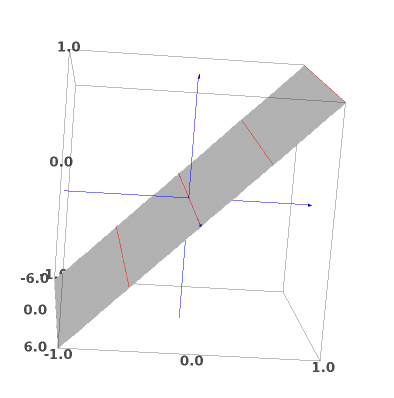
\includegraphics[width=200pt]{qcharacteristic6.png}\end{center}
\caption{The red curves are the characteristic curves parallel to the $x$-axis. The grey surface is the surface traced out by the characteristic curves passing through the initial condition $\phi(0,s)=s$. The initial condition is saying ``pick those characteristic curves which intersect the $x=0$ plane (i.e. the $(y,z)$-plane) at points $y=z$'' which is why the grey surface intersects the $(y,z)$-plane along the diagonal line $y=z$.}
\end{figure}

\section{Example: Burgers's equation}

\begin{exm}\label{exm-burgers-1}
{\bf Solve the equation
\[\frac{\partial\phi}{\partial x}+\phi\frac{\partial\phi}{\partial y}\]
subject to the initial condition $\phi(0,s)=s$.}

We will worry about the initial condition later. This equation has $A(x,y,z)=1$, $B(x,y,z)=z$ and $C(x,y,z)=0$. The characteristic vector field is
\[\left(\begin{array}{c}1\\ z\\ 0\end{array}\right)\]
so a characteristic curve $(x(t),y(t),z(t))$ satisfies
\[\dot{x}=1,\ \dot{y}=z,\ \dot{z}=0.\]
We can solve this and we get
\[z=a,\ y=at+b,\ x=t+c\]
for constants $a,b,c$. For each fixed $a,b,c$ we get a characteristic curve which is a straight line at constant height $a$, with slope $a$ when considered in the $(x,y)$-plane. To get a solution surface we need to pick a one-parameter family of these curves, i.e. we need give $a,b,c$ in terms of a single parameter $s$.

The specification of an initial condition cuts down the amount of choice. In this case the initial condition is $\phi(0,s)=s$. At this is an initial condition, we will impose it at $t=0$ and use it to determine how $a$, $b$ and $c$ depend on $s$. We know that $x=t+c$, $y=at+b$ and $z=a$. Imposing the initial condition means substituting $t=0$, $x=0$, $y=s$ and $z=s$, then solving for $a,b,c$ in terms of $s$. This gives $c=0$ and $a=b=s$. In other words, if we look at the piece of the solution surface living over the line $x=0$ we get a path $s\mapsto(0,s,s)$ in 3-dimensional space which intersects each characteristic curve at the point $t=0$. We call the corresponding characteristic curve $(x(s,t),y(s,t),z(s,t))$ so the map
\[(s,t)\mapsto (t,st+s,s)\]
is the parametrisation of our solution surface.

If we try to find a function $\phi$ such that $z=\phi(x,y)$ on our solution surface then we see that $z=s=y/(t+1)=y/(x+1)$ works. However, this function is not well-defined at $x=-1$. What is happening is that the solution surface fails to be a graph here. Indeed if we draw the projection of the surface to the plane then all of the projections of the characteristic curves cross at the point $(-1,0)$: in $(x,y,z)$-space, the solution surface is becoming vertical over this point and fails to be a graph there.
\end{exm}

\begin{figure}[htb]
\begin{center}
(a)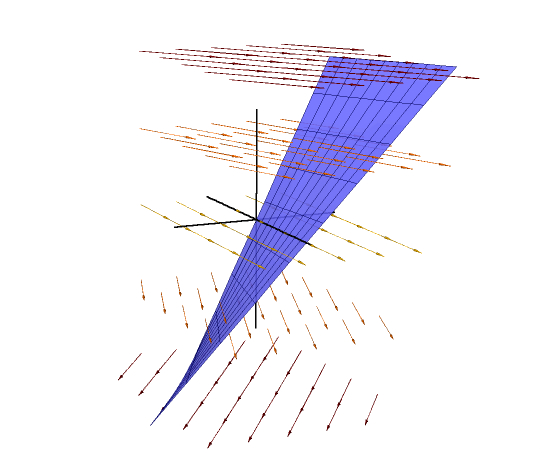
\includegraphics[width=200pt]{quasilinear-characteristics1.jpg} (b)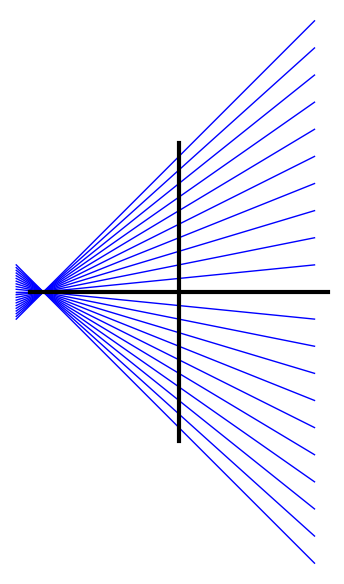
\includegraphics[width=150pt]{qcharacteristics1.png}
\end{center}
\caption{(a) The solution surface to $\frac{\partial\phi}{\partial x}+\phi\frac{\partial\phi}{\partial y}=0$ with the initial condition $\phi(0,y)=y$, plotted with the characteristic vector field. This surface is a union of straight lines which are characteristic curves. (b) The characteristic projections of this solution. You can see that they begin to cross at $(-1,0)$.}
\label{fig-quasilinear-characteristics-1}
\end{figure}

\begin{exm}\label{exm-burgers-2}
{\bf Solve the equation
\[\frac{\partial\phi}{\partial x}+\phi\frac{\partial\phi}{\partial y}\]
subject to the initial condition $\phi(0,s)=s^2$.}

We have the same characteristic curves
\[t\mapsto (t+c,at+b,a)\]
but a different initial condition $\phi(0,s)=s^2$. This gives
\[c=0,\ b=s,\ a=s^2\]
so the solution surface is parametrised by
\[(s,t)\mapsto (t,s^2t+s,s^2).\]
To express $z$ in terms of $x$ and $y$ we have to solve $y=s^2t+s$, $x=t$ for $s$. This gives
\[s=\frac{-1\pm \sqrt{1+4xy}}{2x}\]
or
\[z=\phi(x,y)=\left(\frac{-1\pm \sqrt{1+4xy}}{2x}\right)^2.\]
This fails to be well-defined when $x=0$ or when $1+4xy<0$.

If we draw the projections of the characteristic curves then we can see something strange happening in the vicinity of the curve $1+4xy=0$: the projections start to cross over and bunch up. The solution surface is folding over above this curve so it is not a graph there.
\end{exm}


\begin{figure}[htb]
\begin{center}
(a)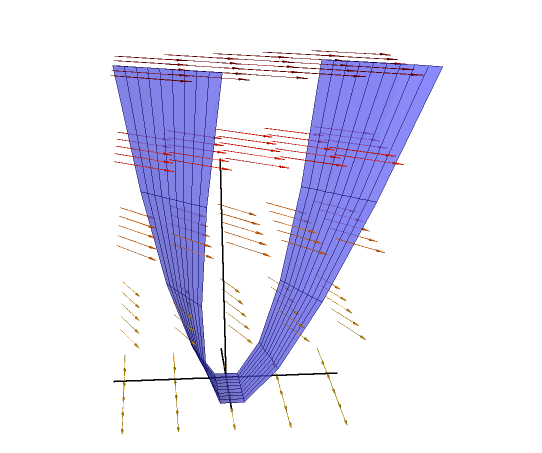
\includegraphics[width=200pt]{quasilinear-characteristics2.jpg} (b)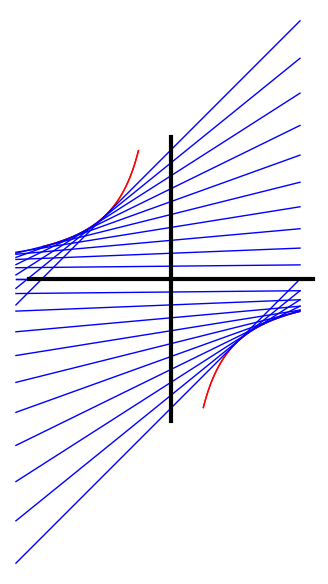
\includegraphics[width=150pt]{qcharacteristics2.png}
\end{center}
\caption{(a) The solution surface to $\frac{\partial\phi}{\partial x}+\phi\frac{\partial\phi}{\partial y}=0$ with initial condition $\phi(0,y)=y^2$, plotted with the characteristic vector field. You can see the graph starting to bend over and become double-valued. (b) The characteristic projections of this solution. You can see that they are all tangent to the red curve $1+4xy=0$ and that they are starting to cross one another near that curve.}
\label{fig-quasilinear-characteristics-2}
\end{figure}
\afterpage{\clearpage}

\section{Caustics}

\begin{dfn}
Let $(s,t)\mapsto(x(s,t),y(s,t),z(s,t))$ be a surface in $\RR^3$. The surface is said to have a vertical tangency at $(x,y,z)$ if some linear combination of the vectors
\[\left(\begin{array}{c}\partial x/\partial s\\\partial y/\partial s\\ \partial z/\partial s\end{array}\right)\mbox{ and }\left(\begin{array}{c}\partial x/\partial t\\\partial y/\partial t\\ \partial z/\partial t\end{array}\right)\]
gives
\[\left(\begin{array}{c}0\\0\\ 1\end{array}\right).\]
Take the set of points where the surface has a vertical tangency and project it to the $(x,y)$-plane. The image is called the {\em caustic} of the surface.
\end{dfn}

\begin{rmk}
The terminology ``caustic'' comes from optics: light travels along rays which are the projections of characteristic curves of a PDE called the eikonal equation. Along the caustic these rays bunch up and give rise to bright patches. The example we studied earlier was Burgers's equation and it arises in the study of waves: $\phi(x,y)$ is the velocity of fluid particles at the point $y$ at time $x$. In this context the caustics are called ``shocks'', where faster fluid particles overtake slower fluid particles.
\end{rmk}

Here is a method for finding the caustic.

\begin{dfn}
If $(s,t)\mapsto (x(s,t),y(s,t),z(s,t))$ is a parametrisation of a surface in $\RR^3$ then consider the projection $\pi(s,t)=(x(s,t),y(s,t))$. A point $(s,t)$ is called a critical point of $\pi$ if the {\em Jacobian determinant}
\[\det\left(\begin{array}{cc}\partial_sx & \partial_sy\\ \partial_tx & \partial_ty\end{array}\right)\]
vanishes. The image under $\pi$ of the set of critical points is called the set $C(\pi)$ of critical values.
\end{dfn}

\begin{lma}
The set $C(\pi)$ of critical values of the projection $\pi$ contains the caustic of the surface.
\end{lma}
\begin{proof}
If a point $(x_0,y_0)$ is in the caustic then there is an $(s,t)$ and coefficients $a,b$ such that
\[a\left(\begin{array}{c}\partial_sx\\\partial_sy\\\partial_sz\end{array}\right)+b\left(\begin{array}{c}\partial_tx\\\partial_ty\\\partial_tz\end{array}\right)=\left(\begin{array}{c}0\\0\\1\end{array}\right).\]
This implies that
\[a\left(\begin{array}{c}\partial_sx\\\partial_sy\end{array}\right)+b\left(\begin{array}{c}\partial_tx\\\partial_ty\end{array}\right)=0\]
so the vectors $\left(\begin{array}{c}\partial_sx\\\partial_sy\end{array}\right)$ and $\left(\begin{array}{c}\partial_tx\\\partial_ty\end{array}\right)$ are linearly dependent. This implies that the Jacobian determinant
\[\det\left(\begin{array}{cc}\partial_sx & \partial_sy\\ \partial_tx & \partial_ty\end{array}\right)\]
vanishes.
\end{proof}
\begin{rmk}
It is not always true that $C(\pi)$ equals the caustic: it is possible for the parametrisation of the surface itself to have a singularity so that the vectors
\[\left(\begin{array}{c}\partial_sx\\\partial_sy\\\partial_sz\end{array}\right)\mbox{ and }\left(\begin{array}{c}\partial_tx\\\partial_ty\\\partial_tz\end{array}\right)\]
are themselves linearly dependent.
\end{rmk}

\begin{exm}
Consider the solution surface $(s,t)\mapsto (t,st+s,s)$ we obtained as a solution to Example \ref{exm-burgers-1}. We have $\pi(s,t)=(t,st+s)$ so that the Jacobian determinant is
\[\det\left(\begin{array}{cc}0 & t+1\\ 1 & s\end{array}\right)=-(t+1).\]
This vanishes when $t=-1$ that is when $x=-1$, $y=0$. This is precisely the bad locus from earlier.
\end{exm}
\begin{exm}
Consider the solution surface $(s,t)\mapsto (t,s^2t+s,s^2)$ we obtained as a solution to Example \ref{exm-burgers-2}. We have $\pi(s,t)=(t,s^2t+s)$ so that the Jacobian determinant is
\[\det\left(\begin{array}{cc}0 & 2st+1\\ 1 & s^2\end{array}\right)=-(2st+1).\]
This vanishes when $2st+1=$, i.e. when $s=-1/2t$. This means $y=1/4t-1/2t=1/4x$, so $4xy+1=0$. This is part of the bad locus from earlier. The other part arose from the solution becoming infinite, not from the solution surface having a vertical tangency.
\end{exm}

\section{Another example}

\begin{exm}
{\bf Solve the PDE
\[-\sin\phi\frac{\partial\phi}{\partial x}+\cos\phi\frac{\partial\phi}{\partial y}=1\]
with initial condition
\[\phi(s,0)=0.\]}

The characteristic vector field is $(-\sin z,\cos z,1)$ and the characteristic curves are
\[z=t+c,\ x=\cos t+a,\ y=\sin t+b\]
These curves are helices spiralling upwards. The initial condition $\phi(s,0)=0$ along $t=0$ gives$c=0$, $s=1+a$, $0=b$ so the solution surface is parametrised by
\[(s,t)\mapsto (\cos t+s-1,\sin t,t).\]
We can express $z$ in terms of $x$ and $y$ easily:
\[z=\sin^{-1}y\]
but this is not a single-valued function so the solution surface is not a graph. If you draw the projections of the characteristic curves you get segments of circles centred on the $x$-axis with radius 1. These all become tangent to the curves $y=\pm 1$ which will turn out to the caustic.

The critical values of the projection are given by the vanishing of the determinant
\[\det\left(\begin{array}{cc}1 & 0\\-\sin t & \cos t\end{array}\right)=\cos t\]
so $t=(n+1/2)\pi$ for some $n\in\mathbf{Z}$. This gives $y=\pm 1$ as expected.
\end{exm}

\begin{figure}[htb]
\begin{center}
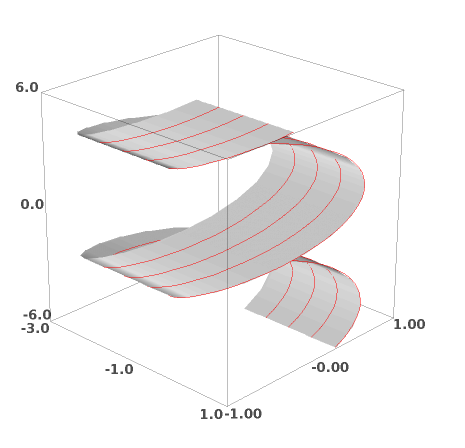
\includegraphics[width=300pt]{qcharacteristics4.png}
\end{center}
\caption{This is the solution surface parametrised by $(\cos t+s-1,\sin t,t)$ and some of the characteristic curves superimposed in red. The surface is folding over itself along the lines $y=\pm 1$.}
\label{fig-characteristics4}
\end{figure}

\begin{figure}[htb]
\begin{center}
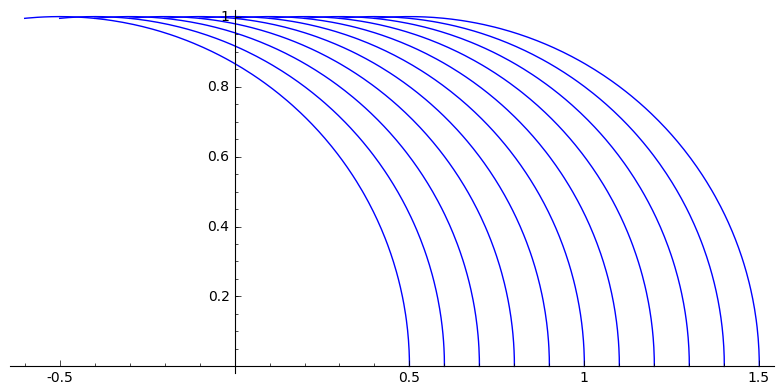
\includegraphics[width=300pt]{qcharacteristics3.png}
\end{center}
\caption{The characteristics of $-\sin\phi\frac{\partial\phi}{\partial x}+\cos\phi\frac{\partial\phi}{\partial y}=1$ are segments of circle. We see they start to overlap near $y=1$.}
\label{fig-characteristics3}
\end{figure}

\chapter[Method of characteristics, III]{* Method of characteristics, III: Fully nonlinear case (NONEXAMINABLE)}

The method works for the fully nonlinear case but the system of ODEs becomes yet more complicated.

\begin{leftbar}
Suppose that $G(x,y,u,p,q)$ is a function of five variables and that $\phi\colon\RR^2\to\RR$ is a function satisfying
\[G\left(x,y,\phi(x,y),\partial_x\phi(x,y),\partial_y\phi(x,y)\right)=0\]
for all $(x,y)\in\RR^2$. Now let $\gamma(t)=(x(t),y(t))$ be a curve and restrict $\phi$ to $\gamma$ to obtain a function $u(t)$ as usual. Let $G(t)$ denote
\[G(x(t),y(t),u(t),p(t),q(t))\]
where $p(t)=\partial_x\phi(x(t),y(t))$, $q(t)=\partial_y\phi(x(t),y(t))$. We have
\[\frac{dG}{dt}=\frac{\partial G}{\partial x}\dot{x}+\frac{\partial G}{\partial y}\dot{y}+\frac{\partial G}{\partial u}\dot{u}+\frac{\partial G}{\partial p}\dot{p}+\frac{\partial G}{\partial q}\dot{q}\]
and since $\dot{u}=\dot{x}\frac{\partial\phi}{\partial x}+\dot{y}\frac{\partial\phi}{\partial y}=\dot{x}p+\dot{y}q$ this becomes
\begin{align*}
\frac{dG}{dt}&=\dot{x}\left(\frac{\partial G}{\partial x}+\frac{\partial G}{\partial u}p\right)+\dot{y}\left(\frac{\partial G}{\partial y}+\frac{\partial G}{\partial u}q\right)+\\
&\ \ \ \ \ +\frac{\partial G}{\partial p}\dot{p}+\frac{\partial G}{\partial q}\dot{q}.
\end{align*}
This suggests a system of five coupled ODEs for the five quantities $(x(t),y(t),u(t),p(t),q(t))$:
\begin{align*}
\frac{dx}{dt}&=\frac{\partial G}{\partial p}&\dot{p}&=-\left(\frac{\partial G}{\partial x}+p\frac{\partial G}{\partial u}\right)\\
\frac{dy}{dt}&=\frac{\partial G}{\partial q}&\dot{q}&=-\left(\frac{\partial G}{\partial y}+q\frac{\partial G}{\partial u}\right)\\
&&\dot{u}&=\frac{\partial G}{\partial p}p+\frac{\partial G}{\partial q}q
\end{align*}
As usual, if we integrate this system of ODEs we will obtain a curve. Taking a one-parameter family of these integral curves gives a surface in $(x,y,u,p,q)$-space and when we project to $(x,y,u)$-space we obtain a surface which, wherever it is a graph, is the graph of a solution $u=\phi(x,y)$.
\end{leftbar}
\begin{figure}[htb]
\begin{center}
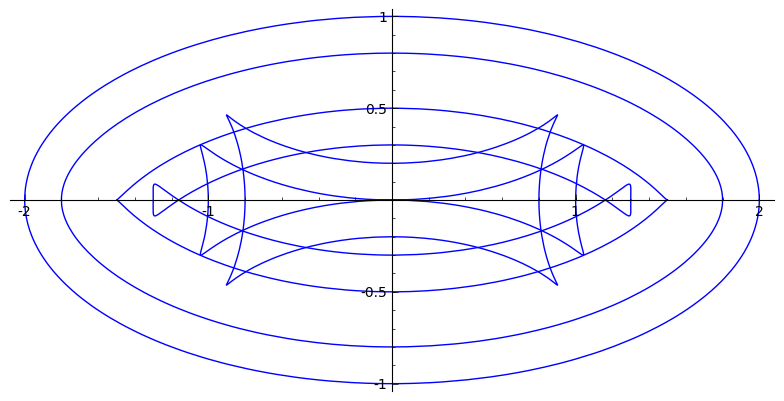
\includegraphics[width=300pt]{equidistants.png}
\end{center}
\caption{The equidistants of an ellipse form singularities as characteristics cross.}
\label{fig-equidistants}
\end{figure}
\begin{leftbar}
\begin{exm}
Let us consider the eikonal equation (in units where the speed of light is 1)
\[\left(\frac{\partial\phi}{\partial x}\right)^2+\left(\frac{\partial\phi}{\partial y}\right)^2=1\]
(so $G(x,y,u,p,q)=p^2+q^2$) which describes the time $\phi$ taken by light emitted normally by some curve $C\subset\RR^2$ to each a point $(x,y)\in\RR^2$. To see that this description is valid, let's consider the corresponding system of ODEs:
\begin{align*}
\frac{dx}{dt}&=2p&\dot{p}&=0\\
\frac{dy}{dt}&=2q&\dot{q}&=0\\
&&\dot{u}&=2(p^2+q^2)=2
\end{align*}
Starting from the curve $C$ and choose the initial condition $\phi|_C=0$. We see that this determines $p$ and $q$ along $C$, namely $(p,q)$ must be (plus or minus) the unit normal vector to the curve $C$ because $p^2+q^2=1$ (giving unit length) and because $(p,q)=\left(\tfrac{\partial\phi}{\partial x},\tfrac{\partial\phi}{\partial y}\right)$ and by our choice of initial condition the directional derivative of $\phi$ along $C$ vanishes, so $(p,q)$ is normal to $C$. Now along the integral curves of the ODE, $p$ and $q$ do not change and hence $x$ and $y$ follow the normal line (with speed 2) and the solution to $\dot{u}=2$ is just $u(t)=2t$. If one followed the normal with speed 1, we would get $u(t)=t$.

This is precisely the statement that the solution of the eikonal equation is the time taken by light to reach $(x,y)$ from $C$ in a normal direction. The characteristics are straight lines normal to $C$. Solutions of the eikonal equation can be very beautiful. Figure \ref{fig-equidistants} shows some of the singularities developed by level sets of $\phi$ corresponding to the initial condition $C=\left\{\frac{x^2}{4}+y^2=1\right\}$ (that is, the equidistants of an ellipse).
\end{exm}
\end{leftbar}


\chapter{D'Alembert's method}

In this final chapter we present one more situation in which a linear change of coordinates enables us to solve a PDE. This time we are interested in linear second-order hyperbolic equations with constant coefficients (and an arbitrary inhomogeneous term).

\section{The wave equation}

The wave equation
\[\frac{1}{c^2}\frac{\partial^2\phi}{\partial t^2}=\frac{\partial^2\phi}{\partial x^2}\]
is supposed to describe the motion of waves with speed $c$. The equation simplifies drastically if we change to so-called {\em light-cone coordinates}:
\[x_+=x+ct,\ x_-=x-ct.\]
The axis $x_-=0$ is a line where $x=ct$, in other words it is the trajectory of a particle moving with speed $c$ in the positive $x$-direction. Similarly the axis $x_+=0$ is the trajectory of a particle moving with speed $c$ in the negative $x$-direction. We have $x=\tfrac{1}{2}(x_++x_-)$ and $t=\tfrac{1}{2c}(x_+-x_-)$. Using the chain rule we have
\begin{align*}
\frac{\partial}{\partial x_{\pm}}&=\frac{\partial x}{\partial x_{\pm}}\frac{\partial}{\partial x}+\frac{\partial t}{\partial x_{\pm}}\frac{\partial}{\partial t}\\
&=\frac{1}{2}\left(\frac{\partial}{\partial x}\pm\frac{1}{c}\frac{\partial}{\partial t}\right)
\end{align*}
so
\[\frac{\partial^2}{\partial x^2}-\frac{1}{c^2}\frac{\partial^2}{\partial t^2}=4\frac{\partial^2}{\partial x_+\partial x_-}.\]
Therefore in these new coordinates the wave equation becomes
\[\frac{\partial^2\phi}{\partial x_+\partial x_-}=0\]
Integrating this directly we see that $\phi(x_-,x_+)=C_-(x_-)+C_+(x_+)$ for arbitrary functions $C_{\pm}$. In other words, {\em any solution to the wave equation can be written as}
\[\phi(x,t)=C_-(x-ct)+C_+(x+ct).\]
We think of the first term as a {\em right-moving wave} and the second as a {\em left-moving wave}. Imagine for example that $C_-=\cos$ and observe that $\cos$ has a local maximum (`crest') at zero. Therefore $C_-(x-ct)$ has a crest at $x-ct=0$, so the crest of this wave moves along the trajectory $x=ct$ of a right-moving particle with speed $c$.

\begin{exm}
{\bf Solve the wave equation for $\phi(x,t)$ with initial conditions}
\[\phi(x,0)=e^{-x^2},\qquad\frac{\partial\phi}{\partial t}(x,0)=0.\]
We know that the solution has the form
\[\phi(x,t)=C_-(x-ct)+C_+(x+ct).\]
The initial conditions become
\[\phi(x,0)=C_-(x)+C_+(x)=e^{-x^2},\qquad\frac{\partial\phi}{\partial t}(x,0)=-cC'_-(x)+cC'_+(x)=0.\]
This gives us two simultaneous equations for $C_{\pm}$. Integrating the second equation implies $C_+(x)=C_-(x)+k$ for some constant $k$. The first then gives
\[C_-(x)+C_+(x)=2C_-(x)+k=e^{-x^2}\]
so $C_-(x)=\frac{1}{2}\left(e^{-x^2}-k\right)$ and $C_+(x)=\frac{1}{2}\left(e^{-x^2}+k\right)$. The solution is therefore
\[\frac{1}{2}\left(e^{-(x-ct)^2}+e^{-(x+ct)^2}\right),\]
in other words, the initial (Gaussian) wave splits into two components with half the amplitude, one moving right, one moving left. Note that the constant $k$ cancelled out. This will always be the case, so we will never bother to include it in our calculations.
\end{exm}

\begin{rmk}[Comparison of Fourier and d'Alembert]
Fourier's (separated) solutions to the wave equation have the form
\[\sin(px)\sin(pct).\]
D'Alembert tells us that we can write this as a sum of a right-moving and a left-moving wave. We can do this explicitly using the trigonometric identities, and we get
\[\sin(px)\sin(pct)=\frac{1}{2}\left(\cos p(x-ct)-\cos p(x+ct)\right).\]
\end{rmk}

\section{Hyperbolic equations}

The wave equation belongs to the class of hyperbolic second-order linear equations. We will consider the most general of these in two variables $x,y$:
\[A\frac{\partial^2\phi}{\partial x^2}+B\frac{\partial^2\phi}{\partial x\partial y}+C\frac{\partial^2\phi}{\partial y^2}=D(x,y)\]
where $A,B,C$ are constants (suppose for simplicity that $A\neq 0$) and $D$ is a function of $x$ and $y$. We will find coordinates $(s,t)$ so that the equation becomes
\[A\frac{\partial^2\phi}{\partial s\partial t}=D\]
in other words, we need to find $(s,t)$ so that
\[A\frac{\partial^2}{\partial s\partial t}=A\frac{\partial^2\phi}{\partial x^2}+B\frac{\partial^2\phi}{\partial x\partial y}+C\frac{\partial^2\phi}{\partial y^2}.\]
The following lemma is good practice in using the chain rule:
\begin{lma}
If we have
\[x=s+t,\qquad y=-\beta s-\alpha t\]
then
\[\frac{\partial^2}{\partial s\partial t}=\frac{\partial^2}{\partial x^2}-(\alpha+\beta)\frac{\partial^2}{\partial x\partial y}+\alpha\beta\frac{\partial^2}{\partial y^2}.\]
\end{lma}
\begin{proof}
We have
\[\frac{\partial}{\partial s}=\frac{\partial x}{\partial s}\frac{\partial}{\partial x}+\frac{\partial y}{\partial s}\frac{\partial}{\partial y}=\frac{\partial}{\partial x}-\beta\frac{\partial}{\partial y}\]
and
\[\frac{\partial}{\partial t}=\frac{\partial x}{\partial t}\frac{\partial}{\partial x}+\frac{\partial y}{\partial t}\frac{\partial}{\partial y}=\frac{\partial}{\partial x}-\alpha\frac{\partial}{\partial y}\]
so
\begin{align*}
\frac{\partial^2}{\partial s\partial t}&=\left(\frac{\partial}{\partial x}-\beta\frac{\partial}{\partial y}\right)\left(\frac{\partial}{\partial x}-\alpha\frac{\partial}{\partial y}\right)\\
&=\frac{\partial^2}{\partial x^2}-(\alpha+\beta)\frac{\partial^2}{\partial x\partial y}+\alpha\beta\frac{\partial^2}{\partial y^2}
\end{align*}
\end{proof}

We will choose $\alpha$ and $\beta$ so that
\[A\frac{\partial^2}{\partial s\partial t}=A\frac{\partial^2}{\partial x^2}+B\frac{\partial^2}{\partial x\partial y}+C\frac{\partial^2}{\partial y^2}\]
that is
\[B/A=-(\alpha+\beta),\qquad C/A=\alpha\beta.\]
\begin{lma}
If $\alpha$ and $\beta$ are the roots of the quadratic equation
\[AT^2+BT+C=0\]
then $B/A=-(\alpha+\beta)$ and $C/A=\alpha\beta$.
\end{lma}
\begin{proof}
The quadratic equation with roots $\alpha$ and $\beta$ and top coefficient $AT^2$ is $A(T-\alpha)(T-\beta)$. Multiplying this out gives $A(T^2-(\alpha+\beta)T+\alpha\beta)$ so $B/A=-(\alpha+\beta)$ and $C/A=\alpha\beta$.
\end{proof}
\begin{dfn}
A PDE
\[A\ppd{\phi}{x}+B\ppdd{\phi}{x}{y}+C\ppd{\phi}{y}=D\]
is said to be hyperbolic, parabolic or elliptic if the quantity $B^2-4AC$ is, respectively, positive, zero or negative.
\end{dfn}
\begin{rmk}
If the PDE is hyperbolic then the roots of $AT^2+BT+C$ are $\tfrac{1}{2A}\left(-B\pm\sqrt{B^2-4AC}\right)$ which are distinct and real. This guarantees that $x=s+t$, $y=-\beta s-\alpha t$ is a well-defined change of coordinates.
\end{rmk}
In conclusion:
\begin{prp}
If
\[A\ppd{\phi}{x}+B\ppdd{\phi}{x}{y}+C\ppd{\phi}{y}=D\]
is a hyperbolic PDE and $\alpha,\beta$ are the roots of $AT^2+BT+C=0$ then under the change of coordinates
\[x=s+t,\qquad y=-\beta s-\alpha t\]
the PDE simplifies to
\[A\ppdd{\phi}{s}{t}=D.\]
\end{prp}

\begin{exm}
{\bf Solve}
\[\frac{\partial^2\phi}{\partial x^2}+5\frac{\partial^2\phi}{\partial x\partial y}+4\frac{\partial^2\phi}{\partial y^2}=xy\]
The quadratic equation we need to solve is $T^2+5T+4=0$ which has roots $(-5\pm\sqrt{25-16})/2$ that is $\alpha=-4$, $\beta=-1$. Under the change of coordinates $x=s+t$, $y=s+4t$ (equivalently $s=\tfrac{1}{3}(4x-y)$, $t=\tfrac{1}{3}(y-x)$) the PDE becomes
\[\frac{\partial^2\phi}{\partial s\partial t}=xy=s^2+5st+4t^2\]
so integrating up directly we get
\[\phi(s,t)=\frac{1}{3}s^3t+\frac{5}{4}s^2t^2+\frac{4}{3}st^3+C_1(s)+C_2(t)\]
where $C_1$ and $C_2$ are arbitrary functions. Changing coordinates back to $x,y$ we have
\begin{align*}
\phi(x,y)&=\frac{1}{81}\left(\frac{1}{3}(4x-y)^3(y-x)+\frac{5}{4}(4x-y)^2(y-x)^2+\frac{4}{3}(4x-y)(y-x)^3\right)\\
&\ \ \ \ \ +C_1((4x-y)/3)+C_2((y-x)/3).
\end{align*}
\end{exm}

\begin{exm}
{\bf Solve}
\[\frac{\partial^2\phi}{\partial x^2}+5\frac{\partial^2\phi}{\partial x\partial y}+4\frac{\partial^2\phi}{\partial y^2}=0\]
{\bf subject to the conditions}
\[\phi(x,0)=x,\qquad\frac{\partial\phi}{\partial y}(x,0)=x^2\]
We have already found the relevant coordinates for this equation in the previous example $s=\tfrac{1}{3}(4x-y)$, $t=\tfrac{1}{3}(y-x)$. With these coordinates the equation becomes
\[\frac{\partial^2\phi}{\partial s\partial t}=0\]
so $\phi(s,t)=C_1(s)+C_2(t)$ or
\[\phi(x,y)=C_1\left(\frac{1}{3}(4x-y)\right)+C_2\left(\frac{1}{3}(y-x)\right).\]
The condition $\phi(x,0)=x$ gives
\[C_1(4x/3)+C_2(-x/3)=x\]
and the condition $\partial\phi/\partial y(x,0)=x^2$ gives
\[-\frac{1}{3}C'_1(4x/3)+\frac{1}{3}C'_2(-x/3)=x^2.\]
Integrating this second equation gives\footnote{Again we are ignoring a constant here because if we included it, it would cancel out later.}
\[-\frac{3}{4}C_1(4x/3)-3C_2(-x/3)=x^3\]
Now we have two simultaneous equations for $C_1$ and $C_2$. These give
\[(3-4/3)C_1(4x/3)=3x+x^3,\qquad (3/4-3)C_2(-x/3)=3x/4+x^3\]
or
\[C_1(4x/3)=4(x^3+3x)/9,\qquad C_2(-x/3)=-4(x^3+3x/4)/9.\]
Substituting $u=4x/3$ we get
\[C_1(u)=u+\frac{3u^3}{16}\]
and substituting $u=-x/3$ we get
\[C_2(u)=u+12u^3.\]
Therefore the final solution, $\phi(s,t)=C_1(s)+C_2(t)$, is
\[\phi(x,y)=\left(\frac{1}{3}(4x-y)+\frac{3}{16}\left(\frac{1}{3}(4x-y)\right)^3\right)+\left(\frac{1}{3}(y-x)+12\left(\frac{1}{3}(y-x)\right)^3\right).\]
\end{exm}

%%% Local Variables: 
%%% mode: latex
%%% TeX-master: "notes"
%%% End: 